% Generated by Listas/make_statements.py from pratica-lecture-06.md, item 26. Do not edit.
\textbf{Source.} Tadelis (2013), \emph{Game Theory: An Introduction}, Exercise 10.10 ``Law Merchants Revisited'', p.~219 {[}PDF 238{]}. Reproduced verbatim. Figure 10.2 (p.~206) is not part of the exercise text; it is added because Section 10.5.2, which the statement cites, builds the game on it. Answer in the source: none in the book (the preface, p.~xiii, says about half are solved on Princeton UP's website; not checked).



\begin{quote}

\textbf{Law Merchants Revisited:} Consider the three-person game described in Section 10.5.2. A subgame-perfect equilibrium was constructed with a bond equal to 2, a fee equal to \(w = 0.1\) was paid by every player \(P_2^t\) to player 3, and it was shown that it is indeed an equilibrium for any discount factor \(\delta \ge 0.95\). Show that a similar equilibrium exists in which players \(P_1^t\) trust players \(P_2^t\) who post bonds, players \(P_2^t\) post bonds and cooperate, and player 3 follows the contract in every period, for any discount factor \(0 < \delta < 1\).

\end{quote}



\pandocbounded{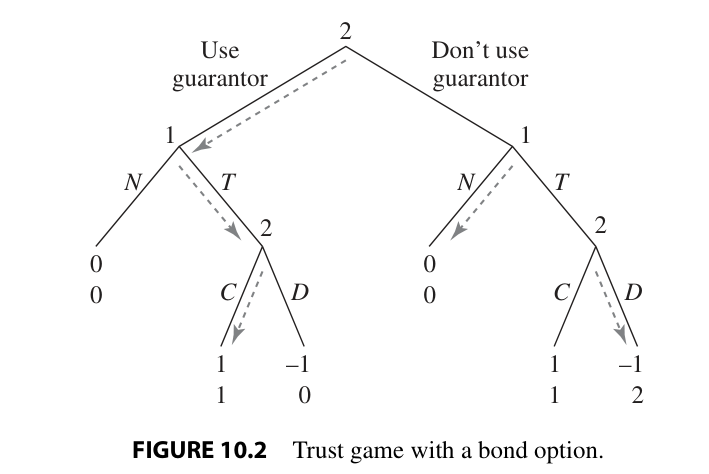
\includegraphics[keepaspectratio,alt={Tadelis Figure 10.2, the trust game with a bond option}]{../figures/tadelis-fig-10-2.png}}



\emph{Figure 10.2} Trust game with a bond option (Tadelis p.~206; added for reference).

